%%%%%%%%%%%%%%%%%%%%%%%%%%%%%%%%%%%%%%%%%%%%%%%%%%%%%%%%%%%
% Capitolo 1

\chapter{Implementazione ed utilizzo}
\label{ref:test}

Dopo la fase di sviluppo, l'applicazione sarà disponibile per tutti i dispositivi Windows Phone tramite il Windows Store, ovvero l'insieme delle applicazioni certificate da Microsoft ed installabili su tutti i cellulari della famiglia.
Prima di questa fase, si è effettuata una fase di verifica sul campo.

L'applicazione \textbf{VisitPaestum} è stata testata nel sito archeologico degli scavi di Paestum.
Questa fase è finalizzata a verificare quelle funzionalità strettamente legate ad un ambito di utilizzo all'aperto, perché le altre funzionalità riportate nel capitolo 3 sono state verificate durante la fase di sviluppo e con l'applicazione eseguita dall'emulatore compreso nell'SDK.

Il server che fornisce i dati ai client è stato realizzato, in modalità prototipale, tramite un approccio Cloud che si è basato sulla tecnologia Microsoft Azure: in questo modo si è potuto avere a disposizione un server accessibile dalla rete Internet con costi di installazione ed utilizzo particolarmente ridotti.

Dopo l'avvio dell'applicazione, cliccando sul pulsante per la visualizzazione dei punti di interesse (l'ultimo pulsante a destra sulla barra) si visualizzano delle icone a forma di tempio dove sono i punti di interesse, come visualizzato in figura \ref{visualizzazionepuntidiinteresse}.
\begin{figure}[h!]
\begin{center}
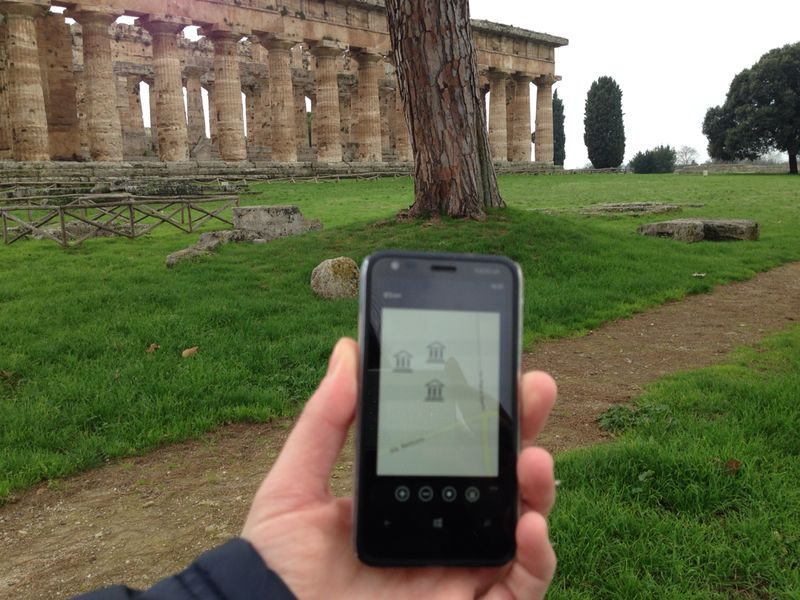
\includegraphics[scale=0.4]{imgs/immaginiapp/visualizzazionepuntidiinteresse.jpg} 
\caption{Screenshot dell'applicazione con visualizzazione dei punti di interesse.\label{visualizzazionepuntidiinteresse}}
\end{center}
\end{figure}

Cliccando su uno dei punti di interesse, si può accedere al menu contestuale, come si può visualizzare in figura \ref{visualizzazionemenu}.
\begin{figure}[h!]
\begin{center}
\includegraphics[scale=0.4]{imgs/immaginiapp/visualizzazionemenu.jpg} 
\caption{Screenshot dell'applicazione con visualizzazione del menu contestuale.\label{visualizzazionemenu}}
\end{center}
\end{figure}
Tramite il menu contestuale, è possibile visualizzare i dettagli relativi al punto di interesse selezionato, visualizzare i feedback ricevuti e rilasciarne uno.

Cliccando su "Inserisci feedback", è possibile inserire un feedback per il punto di interesse selezionato, come mostrato in figura \ref{inserimentofeedback}.
\begin{figure}[h!]
\begin{center}
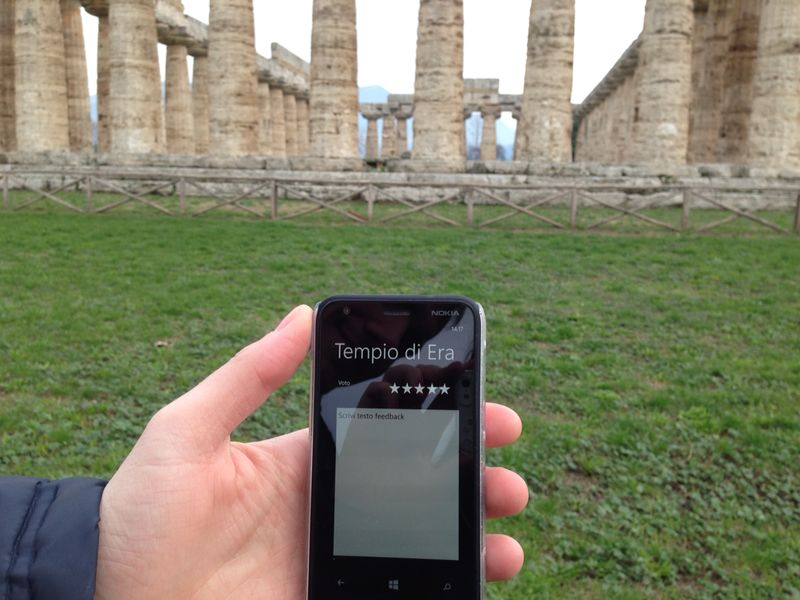
\includegraphics[scale=0.4]{imgs/immaginiapp/inserimentofeedback.jpg} 
\caption{Screenshot dell'applicazione per l'inserimento del feedback.\label{inserimentofeedback}}
\end{center}
\end{figure}

Spostandoci nei pressi del tempio di Era, il servizio di localizzazione che opera in background ci mostra a video (figura \ref{tempiodiera}) la pagina di dettaglio di questo Tempio, al fine di mostrare le informazioni più importanti.
\begin{figure}[h!]
\begin{center}
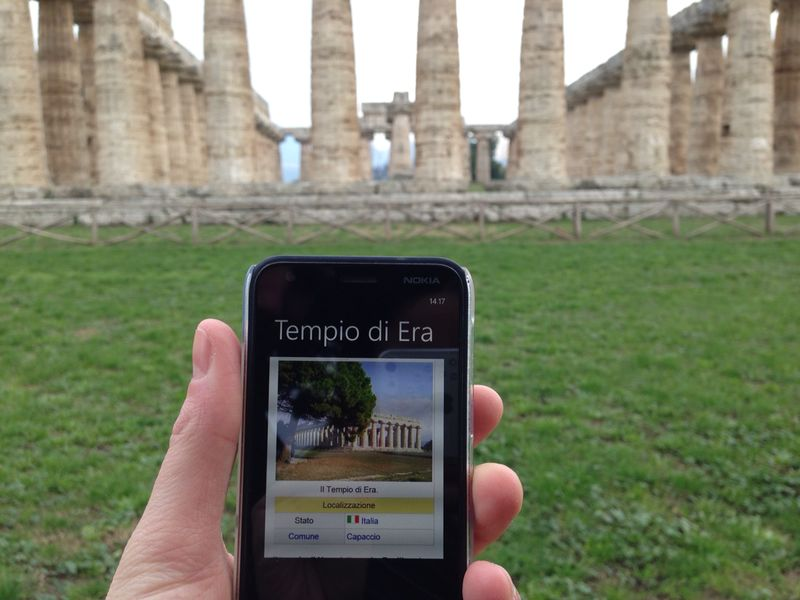
\includegraphics[scale=0.4]{imgs/immaginiapp/tempiodiera.jpg} 
\caption{Screenshot dell'applicazione con visualizzazione delle informazioni del tempio di Era.\label{tempiodiera}}
\end{center}
\end{figure}


Allo stesso modo, spostandoci nei pressi del tempio di Nettuno, il servizio di localizzazione che opera in background ci mostra a video (figura \ref{tempiodinettuno}) la pagina di dettaglio di questo tempio con le informazioni più importanti.

\begin{figure}[h!]
\begin{center}
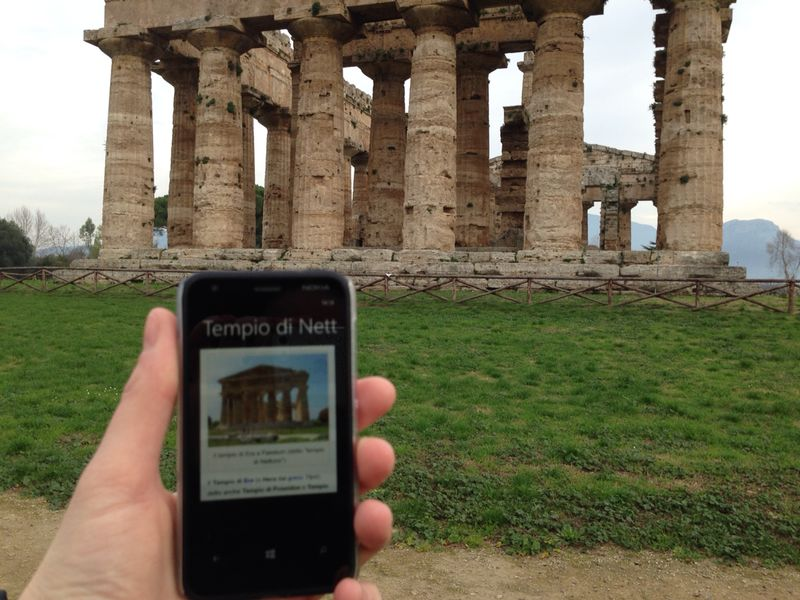
\includegraphics[scale=0.4]{imgs/immaginiapp/tempiodinettuno.jpg} 
\caption{Screenshot dell'applicazione con visualizzazione delle informazioni del tempio di Nettuno.\label{tempiodinettuno}}
\end{center}
\end{figure}


%%%%\clearpage{\pagestyle{empty}\cleardoublepage}